%!TEX root = ../../main.tex
%----------------------------------------------------------------------------
\chapter{Robot Cell Design}\label{chap:robot_cell_chapter}
%----------------------------------------------------------------------------

Each team was provided with one robot cell, equipped with a Kuka KR 6 manipulator and a conveyor belt. After the mobile platform has carried out its delivery order, the LEGO bricks are dumped on the conveyor belt, which moves them in reach of the manipulator, which then attempts to recognize them and select the ones on its order list issued by the MES server. The selected ones are then packed, while the remainder is placed in a box. This is the task each robot cell has to fulfill, and just like in the case of the mobile platform, the process can be subdivided into smaller tasks, which we will introduce in the upcoming sections.



% Please keep sections separated in their designated folders and only reference them here using the input tag

%!TEX root = ../../../main.tex
%%---------------------------------------------------------------------------
\section{Conveyor Belt Controller} 
\label{sec:conveyor_belt_sec}
%%---------------------------------------------------------------------------
The conveyor belt is driven by an AC motor and requires a frequency generator in order to move. The provided frequency generator can either be manually controlled or by a $24V$ digital interface. The interface between the controlling computer and the frequency generator is a PLC. A PLC is an industrial \textit{computer} with $24V$ IO interface and is logic driven. This can be programmed in different ways such as Ladder Diagrams, Structured Text and Function Block Diagrams.\\ 

The PLC in this project is programmed in Structured Text and is simply set up to respond to some serial commands. This makes it possible to start, stop and change the direction of the conveyor belt from an external serial connection.
%%---------------------------------------------------------------------------
\section{Brick Detection \label{sec:brick_detection_sec}}
%%---------------------------------------------------------------------------

Details on how the bricks are detected and selected for sorting. (How, how well)

%!TEX root = ../../../main.tex
%%---------------------------------------------------------------------------
\section{Manipulator Control \label{sec:manipulator_control_sec}}
%%---------------------------------------------------------------------------

Description of how the Kr 6 is being controlled, and how the grasping was implemented.

%!TEX root = ../../../main.tex
%%---------------------------------------------------------------------------
\section{Human Machine Interface}
\label{sec:rc_hmi}
%%---------------------------------------------------------------------------
A separate Human Machine Interface (HMI) is developed for controlling the robot cell. This allows the user to control relevant parameters from an intuitive GUI. 

The HMI is implemented as a plugin to RobWorkStudio. This allows the HMI to act alongside the visual representation of the work-cell allowing a real-time simulation of the actions.

Figure \ref{fig:rc_hmi} shows the HMI plugin. All system elements are using the log for error and information messages. The user is able to manually control the robot, conveyor and gripper. Some camera settings can be directly controlled from the HMI and the video feed shows a direct view of either the raw or vision applied image. 

	\begin{figure}[H]
		\centering
	    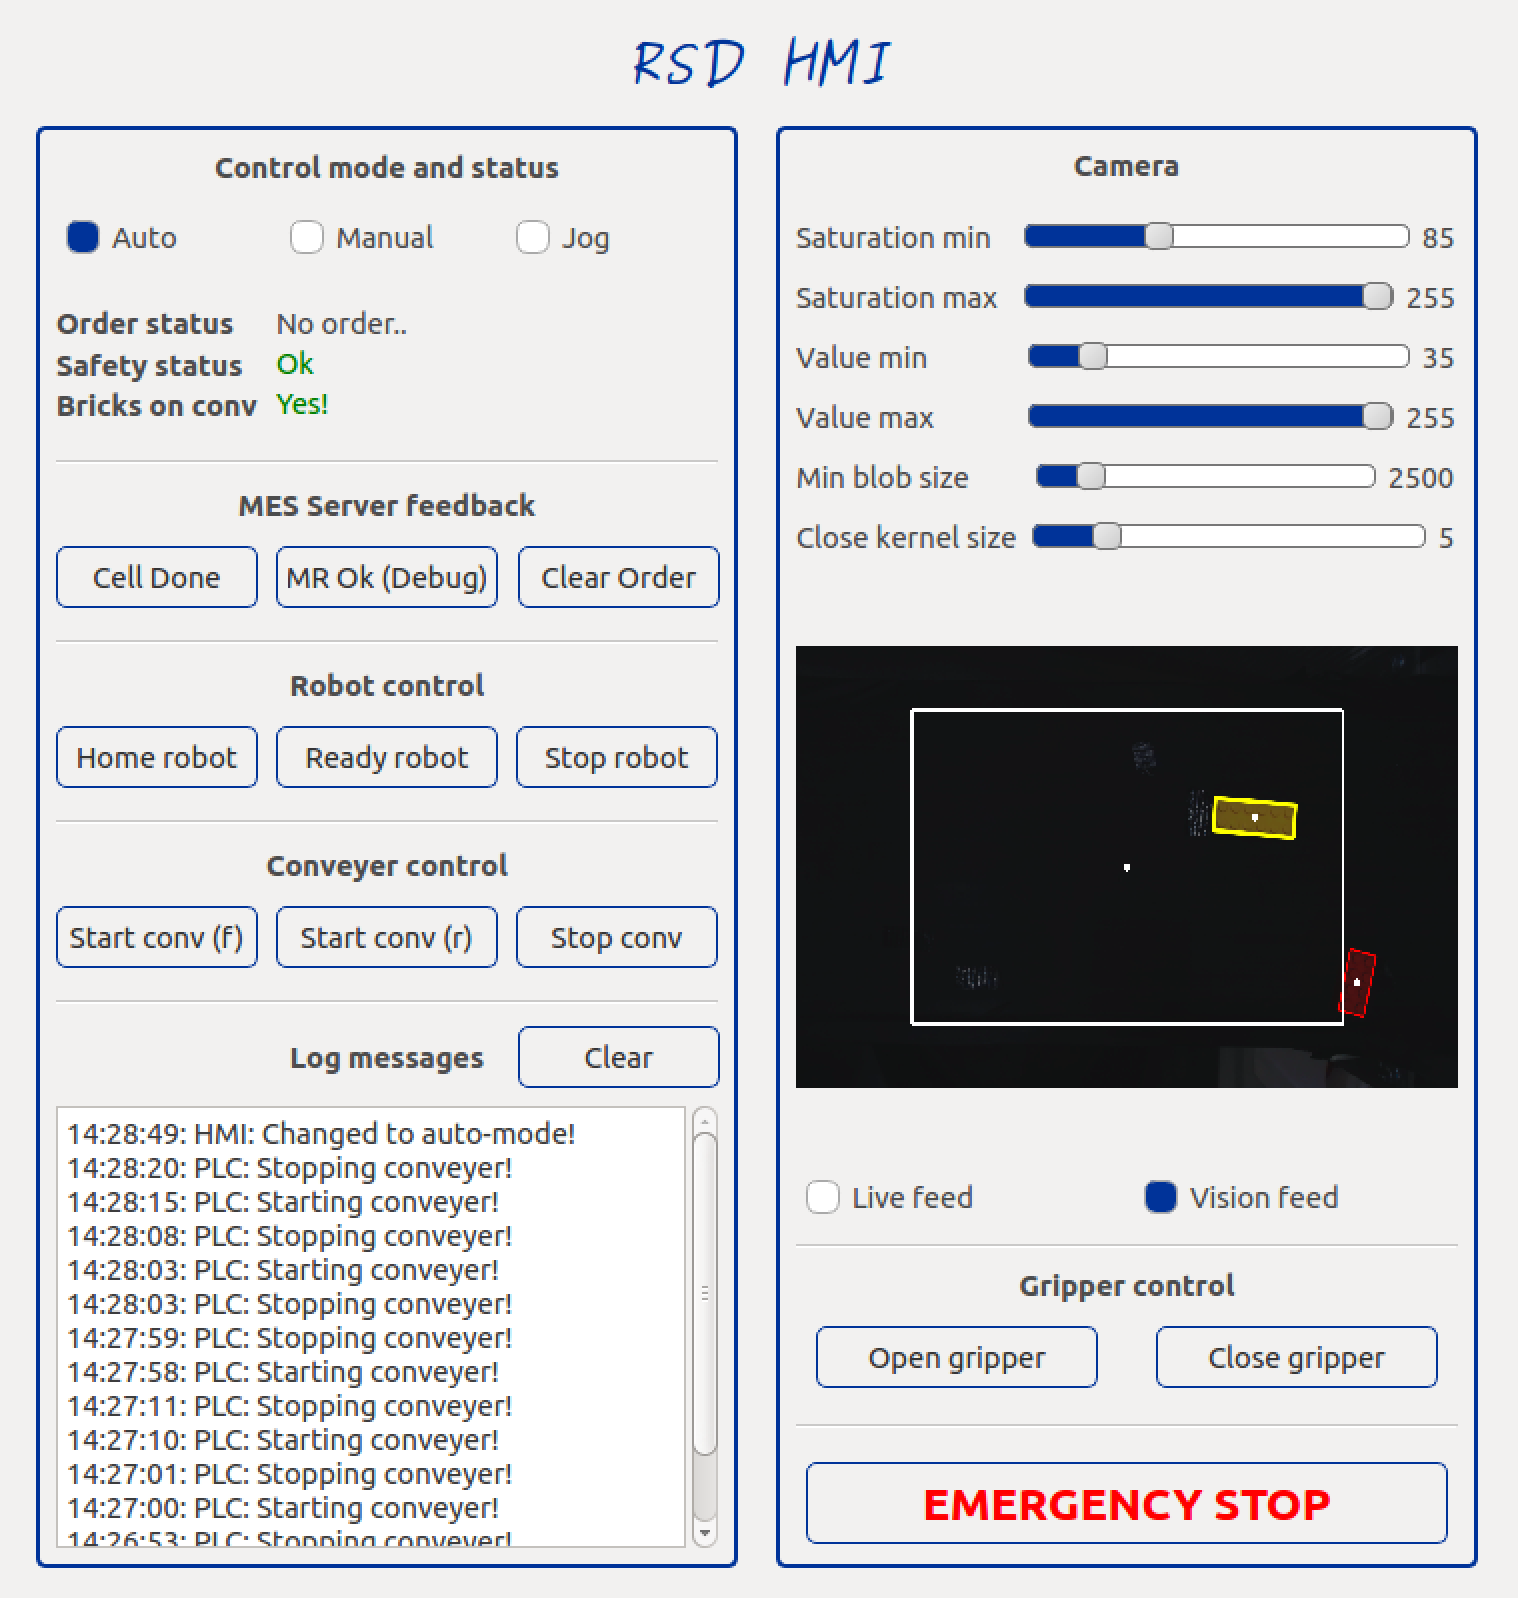
\includegraphics[width=0.9\textwidth]{rc_hmi}
	    \caption{HMI}
		\label{fig:rc_hmi}
	\end{figure}



%%% Local Variables:
%%% mode: latex
%%% TeX-master: "main"
%%% End: